\documentclass[11pt,a4paper]{article}
\usepackage[margin=2.4cm]{geometry}
\usepackage{times}
\usepackage{amsmath,amssymb}
\usepackage{graphicx}
\usepackage{booktabs}
\usepackage{tabularx}
\usepackage{siunitx}
\usepackage{hyperref}
\usepackage{natbib}
\usepackage{setspace}
\usepackage{caption}
\usepackage{subcaption}
\onehalfspacing
\hypersetup{colorlinks=true,linkcolor=blue,citecolor=blue,urlcolor=blue}
\captionsetup{font=small,labelfont=bf}

\title{Matched-Capacity Hybrid Quantum-Classical Networks for Confidence Calibration under Cross-Population Chest X-Ray Shift}
\author{Tran Thi Thuy Quyen\\
Information Assurance, FPT University Can Tho, Vietnam\\
\texttt{alwayshavebeenyaa@gmail.com}}
\date{}

\begin{document}
\maketitle

\begin{abstract}
Hybrid quantum-classical networks are often presented as replacements for convolutional classifiers. That comparison is not well posed when a parameterized quantum circuit (PQC) consumes a handful of engineered scalars while the classical baseline consumes the full image. This paper asks a narrower question that the implementation can answer. On a shared six-dimensional bottleneck taken from a frozen ImageNet DenseNet-121, does a PQC change discrimination or confidence calibration relative to a capacity-matched multilayer perceptron (MLP) when models trained on CheXpert (United States) are evaluated on VinDr-CXR (Vietnam)? Three heads are trained: an MLP, a product PQC without entangling gates, and an entangling PQC with a CNOT ring. All heads map six angle-embedded features to a single logit; the PQC measures $\langle Z\rangle$ on qubit~0. Forty-five runs (five tasks $\times$ three heads $\times$ three seeds) are reported. On CheXpert test data, PQC heads do not outperform the MLP on AUROC. Entanglement does not systematically reduce expected calibration error (ECE). Temperature scaling fitted on CheXpert validation logits can lower source ECE and raise target ECE on the same run. VinDr-CXR has no Pneumonia class; a pneumonia proxy (Consolidation $\cup$ Infiltration) is an ontology shift and is confined to the appendix. At this capacity, on a noiseless simulator, a PQC is not a more trustworthy head under cross-population shift. That empirical boundary is the result.
\end{abstract}

\noindent\textbf{Keywords:} confidence calibration; domain shift; chest radiography; parameterized quantum circuit; matched capacity

\section{Introduction}

A chest-radiograph classifier that looks well calibrated in one hospital can become over- or under-confident in another~\citep{ovadia2019shift,zech2018variable}. Calibration under shift is therefore a clinical property, not a training curiosity. In parallel, variational quantum circuits have been attached to classical backbones and described as hybrid quantum-classical networks~\citep{benedetti2019pqc,cerezo2021vqa}. Many of those studies compare a small PQC with a fully trained convolutional classifier, or they collapse label ontologies across datasets in order to claim a cross-site pneumonia detector. Both moves inflate the apparent role of the circuit.

The model studied here, Q-CalibNet, is deliberately smaller than that rhetoric. A DenseNet-121~\citep{huang2017densenet} pretrained on ImageNet~\citep{deng2009imagenet} is frozen and used only as a 1024-dimensional feature extractor. A linear map compresses those features to six $\tanh$-scaled angles. Three heads of nearly equal parameter count then produce a binary logit: a two-layer MLP (6\,215 trainable parameters, including the bottleneck), a product PQC, and an entangling PQC (6\,188 parameters each). The research questions follow the code.

\begin{itemize}
\item \textbf{RQ1 (secondary).} On the same six-dimensional bottleneck, do product or entangling PQCs differ from the MLP in AUROC, AUPRC, or F1 when models trained on CheXpert are evaluated on VinDr-CXR?
\item \textbf{RQ2 (primary).} Does entanglement reduce ECE, maximum calibration error (MCE), Brier score, or overconfidence under shift, relative to a product PQC and the MLP?
\item \textbf{RQ3.} Does a scalar temperature fitted on CheXpert validation logits calibrate PQC heads more effectively than the MLP on the Vietnamese target?
\end{itemize}

The contribution is the protocol, not a supremacy claim. Capacity is matched. Product versus entangling circuits isolate the inductive bias of CNOT. CheXpert uncertain labels are dropped (U-Ignore)~\citep{irvin2019chexpert}. VinDr multi-radiologist boxes are reduced with an any-vote~\citep{nguyen2022vindrcxr}. Tasks with a shared finding name are reported in the main tables; pneumonia is not.

\section{Related work}

\subsection{Confidence calibration}

A probabilistic classifier is calibrated when, among instances predicted with confidence $p$, the empirical frequency of the predicted event is also $p$. \citet{brier1950verification} introduced a proper scoring rule that jointly penalizes discrimination and calibration. \citet{naeini2015ece} defined expected calibration error by binning confidence and averaging the absolute gap between accuracy and confidence; \citet{nixon2019measuring} later documented the sensitivity of that estimator to binning. \citet{platt1999probabilistic} and \citet{zadrozny2002transforming} treated calibration as a post-hoc map from scores to probabilities. \citet{guo2017calibration} showed that modern deep networks are systematically overconfident and that a single temperature $T$ fitted by negative log-likelihood on a validation set---temperature scaling---is a strong, almost parameter-free baseline. \citet{kull2019dirichlet} generalized the idea to Dirichlet calibration in the multi-class setting. None of these methods assumes that the validation distribution matches the deployment distribution. \citet{ovadia2019shift} showed that predictive uncertainty, including temperature-scaled confidence, degrades under covariate and semantic shift. The present study uses Guo-style scalar temperature as RQ3, fitted only on CheXpert validation logits, and tests whether that $T$ transfers to VinDr-CXR.

\subsection{Chest radiography, labels, and shift}

Large CXR corpora made convolutional screening feasible and also made dataset shift visible. ChestX-ray8~\citep{wang2017chestxray8}, CheXpert~\citep{irvin2019chexpert}, MIMIC-CXR~\citep{johnson2019mimiccxr}, and VinDr-CXR~\citep{nguyen2022vindrcxr} differ in geography, devices, report style, and label generation. CheXNet~\citep{rajpurkar2017chexnet} reported radiologist-level pneumonia detection on a single corpus; subsequent analyses showed that such numbers need not travel. \citet{zech2018variable} documented hospital-specific shortcuts in pneumonia CNNs. \citet{oakden2020hidden} described hidden stratification: a high AUROC can hide failure on clinically important subtypes. \citet{seyyed2021underdiagnosis} showed underdiagnosis bias in underserved groups. \citet{pooch2020shift} measured domain shift among CXR classifiers directly. CheXpert encodes uncertainty as $-1$ and defines U-Ignore, U-Ones, and U-Zeros~\citep{irvin2019chexpert}; collapsing those conventions, or mapping CheXpert Pneumonia onto VinDr classes that do not include Pneumonia, is an ontology change rather than a population change. VinDr-CXR provides box annotations from multiple radiologists on 15\,000 training radiographs collected in Vietnam~\citep{nguyen2022vindrcxr}. The present protocol keeps U-Ignore, uses an any-vote on VinDr boxes, reports four overlapping findings in the main table, and isolates Consolidation $\cup$ Infiltration as an appendix proxy.

\subsection{Parameterized quantum circuits as models}

Parameterized quantum circuits are variational models whose gates carry trainable angles~\citep{mitarai2018qcl,benedetti2019pqc,cerezo2021vqa}. Angle embedding of a classical vector, followed by layers of single-qubit rotations and optional entangling gates, is the default encoding in several software stacks, including PennyLane~\citep{bergholm2018pennylane}. \citet{schuld2019feature} and \citet{havlicek2019supervised} framed such circuits as feature maps into Hilbert space. \citet{schuld2021encoding} showed that the encoding---not only the variational block---controls the Fourier spectrum of the hypothesis class. \citet{perez2020reuploading} showed that re-uploading data can make even a single qubit a universal classifier in theory. Expressibility and entangling capability of common ansatze were quantified by \citet{sim2019expressibility}. Those capacity measures do not imply better calibration. Training is further constrained by barren plateaus~\citep{mcclean2018barren}. \citet{huang2021powerdata} and \citet{abbas2021power} argued that quantum models can be powerful, but that classical data and geometric differences, not circuit depth alone, decide advantage. The implication for CXR work is prosaic: a six-qubit expectation head on a frozen DenseNet vector is a small classical-to-quantum map. Comparing it with a fully trained DenseNet classifier confounds representation learning with the head. Comparing a product circuit with an otherwise identical CNOT-ring circuit does not.

\subsection{What this paper does not claim}

This paper does not claim quantum advantage, hardware execution, or state-of-the-art CXR detection. It does not treat the unmatched DenseNet classifier as a fair baseline. It does not merge pneumonia across ontologies in the primary table. Related hybrid-imaging papers that do those things are not used as performance targets.

\section{Methods}

\subsection{Source and target}

CheXpert-v1.0-small is the source~\citep{irvin2019chexpert}. Only frontal radiographs are kept. Uncertain labels ($-1$) are dropped; blank findings are treated as negative, matching the CheXpert competition convention. Splits are patient-level. Training uses 2\,000 class-balanced images; validation and test use 500 images at natural prevalence (Table~\ref{tab:splits}).

VinDr-CXR / VinBigData training images (15\,000 PNG files) are the external target~\citep{nguyen2022vindrcxr}. Labels come from the public box CSV. An image is positive for a finding if any radiologist assigned that class. No VinDr image is used for training. Two holdouts of 1\,000 images are built: a class-balanced set and a natural-prevalence set. Consolidation has only 353 positives in the entire VinDr training set, so the ``balanced'' holdout is 353/647 rather than 500/500. The 3\,000-image Kaggle test split has no public labels and is unused.

\subsection{Tasks}

Four primary tasks share a finding name on both datasets: no finding, cardiomegaly, pleural effusion, and consolidation. No finding is the cleanest ontology (positive $=$ absence of any recorded abnormality). A fifth task, \texttt{pneumonia\_proxy}, maps CheXpert Pneumonia to VinDr Consolidation $\cup$ Infiltration and is flagged \texttt{ontology\_shift=True}. It is not a pneumonia detector and is not used to claim cross-dataset pneumonia performance.

\subsection{Architecture}

Let $x \in \mathbb{R}^{1024}$ be the frozen DenseNet-121 feature. The bottleneck is
\begin{equation}
z = \pi \tanh(Wx + b) \in \mathbb{R}^{6}.
\end{equation}
The MLP head is $6 \to 8 \to \tanh \to \mathrm{Dropout}(0.1) \to 1$. Each PQC uses six wires, two layers of RX/RY/RZ, and $Y$-angle embedding of $z$~\citep{schuld2021encoding,bergholm2018pennylane}. The product circuit has no CNOTs; the entangling circuit adds a CNOT ring after each rotation layer~\citep{sim2019expressibility}. The readout is $\mathrm{scale}\cdot\langle Z_0\rangle + \mathrm{bias}$. The bottleneck tensor is not detached: gradients flow into $W$ for every head, which is the condition under which the comparison remains matched-capacity. Circuits are simulated with PennyLane \texttt{default.qubit} and backpropagation on CPU float64. There is no hardware run and no claim that six qubits process a $1024\times 1024$ radiograph.

\subsection{Training and calibration}

Heads are trained with Adam~\citep{kingma2015adam} ($\mathrm{lr}=10^{-3}$, weight decay $10^{-4}$), binary cross-entropy with logits, 40 epochs, and early stopping of 8 epochs on validation AUROC~\citep{hanley1982roc}. MLP batches are size 64 on CUDA; PQC batches are size 16 on CPU. Seeds are 42, 43, and 44. After training, a scalar temperature $T=\exp(\theta)$ is fitted by L-BFGS on CheXpert validation logits~\citep{guo2017calibration}, with $T$ clamped to $[10^{-3}, 100]$. Calibrated probabilities use $\sigma(\mathrm{logit}/T)$. Metrics: AUROC, AUPRC~\citep{davis2006pr}, F1 at 0.5, Brier score~\citep{brier1950verification}, and 15-bin ECE and MCE~\citep{naeini2015ece,guo2017calibration}. JSON records do not store logits; reliability diagrams are recomputed from checkpoints. A run is called $T$-degenerate if the optimizer hit the clamp. Those seven runs are retained in the main table and removed only in a sensitivity ablation.

\subsection{What is not compared}

A fully trained DenseNet classifier is an unmatched upper bound. Fine-tuning the backbone, adding qubits mid-grid, merging pneumonia with consolidation in the main table, or describing PQC AUROC as quantum advantage would break the protocol.

\section{Results}

Forty-five of forty-five scheduled runs finished. VinDr metrics are present for every run. Mean $\pm$ standard deviation is over three seeds. Degenerate temperatures occurred on seven runs and are retained.

\subsection{RQ1: discrimination}

On CheXpert test data, the MLP is at least as discriminative as either PQC on every primary task (Table~\ref{tab:primary}; Fig.~\ref{fig:bars}). For no finding, AUROC is $0.837\pm 0.003$ (MLP), $0.820\pm 0.007$ (product), and $0.813\pm 0.010$ (entangling). Under VinDr balanced evaluation, AUROC falls for no finding (MLP $0.736\pm 0.008$, product $0.669\pm 0.003$, entangling $0.725\pm 0.015$). Product PQC is not uniformly worse on the target: on consolidation its VinDr AUROC is $0.714\pm 0.012$ against MLP $0.682\pm 0.035$, inside seed noise and below any claim of advantage. Cardiomegaly product seed 43 is an outlier (CheXpert AUROC $0.596$). Across 12 primary task--seed pairs, product AUROC is below the matched MLP on 9 CheXpert tests; entangling AUROC is below the MLP on 10. Three seeds do not support a hierarchical significance test; the pattern is reported as paired mean differences, not as $p$-values.

\subsection{RQ2: entanglement and calibration}

Entangling circuits do not yield lower source ECE (Table~\ref{tab:primary}; Fig.~\ref{fig:bars}). For no finding, CheXpert test ECE is $0.320\pm 0.069$ (MLP), $0.239\pm 0.031$ (product), and $0.379\pm 0.038$ (entangling). The entangling head on no finding seed 42 is the clearest single-run illustration: test accuracy $0.56$, sensitivity $0.95$, ECE $0.419$ (Fig.~\ref{fig:reliability}). Ring CNOTs at two layers and a single-qubit readout are not a calibration regularizer in this regime. On VinDr balanced data, raw ECE is sometimes lower for PQC heads, but that reduction coexists with weaker or comparable AUROC and does not survive temperature transfer.

\subsection{RQ3: temperature transfer}

Temperature fitted on CheXpert validation is not a reliable target calibrator (Fig.~\ref{fig:transfer}). On no finding product PQC, mean CheXpert ECE falls after scaling ($0.239\to 0.153$) while VinDr balanced ECE rises ($0.124\to 0.203$). Seed 43 of that head is extreme: $T=0.36$ reduces CheXpert ECE from $0.212$ to $0.054$ and increases VinDr balanced ECE from $0.123$ to $0.259$. Seven runs hit the clamp ($T=100$ or $T=0.001$); those fits flatten or sharpen probabilities until ECE on one domain is an artifact of the box constraint. Dropping them does not reverse RQ1 or RQ2 on no finding or pleural effusion, where no run was degenerate. The honest statement of RQ3 is negative: source-fitted $T$ does not systematically help PQC more than MLP on VinDr-CXR. This is consistent with~\citet{ovadia2019shift}: a validation-fitted uncertainty map need not travel.

\subsection{Appendix task}

\texttt{pneumonia\_proxy} CheXpert test prevalence is $0.024$ (12 positives in 500). AUROC numbers on that split are high-variance and are not pneumonia performance. They are reported in Table~\ref{tab:appendix} only to show that an ontology collapse would have been easy to overclaim.

\section{Limitations}

The circuit has six qubits, two layers, and a single observable. The backbone is frozen, so the PQC never sees pixels. Simulation uses \texttt{default.qubit}, not hardware noise. Sample sizes are small (train 2\,000; val/test 500; VinDr 1\,000). Three seeds cannot support a confirmatory hypothesis test. Temperature is a scalar with a hard clamp. ECE uses 15 equal-width bins; rare positives make several bins empty~\citep{nixon2019measuring}. VinDr any-vote ignores radiologist disagreement. ImageNet-normalized $224\times 224$ RGB conversion is a crude CXR preprocessing. None of these limitations is hidden in order to protect a quantum narrative.

\section{Conclusion}

Matched-capacity hybrid heads on a six-dimensional CXR bottleneck do not produce a more trustworthy classifier under CheXpert $\to$ VinDr-CXR shift. Discrimination is comparable or slightly worse for PQC than for an MLP. Entanglement does not reduce ECE. Temperature scaling fitted on the source can harm the target. Those are reportable empirical boundaries. They are not evidence against quantum machine learning in general; they are evidence against overclaiming a six-qubit expectation head as a cross-population calibrator.

\section*{Reproducibility}

Code and configs live with the project. Interpreter: Python 3.10, PyTorch 2.6.0+cu124, PennyLane 0.38.0. Grid: \texttt{scripts/run\_queue.py}. Tables: \texttt{results/tables/all\_runs.csv}. Figures: \texttt{results/figures/}. Checkpoints: \texttt{results/runs/}. Splits were not resampled after the grid. Logits for reliability diagrams are dumped from checkpoints by \texttt{scripts/dump\_logits.py}.

\section*{Ethics}

CheXpert and VinDr-CXR are public de-identified research datasets. No clinical deployment is claimed. The author has no competing interests.

\bibliographystyle{plainnat}
\bibliography{references}

\appendix
\section{Split prevalences}
\label{tab:splits}
\begin{table}[h]
\centering
\small
\caption{Evaluation-split sizes after the frozen protocol (not resampled). Train is class-balanced at $n=2000$ for every task.}
\begin{tabular}{lrrrrrr}
\toprule
Task & CheXpert test $n_+$ & prev. & VinDr-bal $n_+$ & prev. & VinDr-nat $n_+$ & prev. \\
\midrule
No finding & 41 & 0.082 & 500 & 0.500 & 702 & 0.702 \\
Cardiomegaly & 63 & 0.126 & 500 & 0.500 & 164 & 0.164 \\
Pleural effusion & 225 & 0.450 & 500 & 0.500 & 62 & 0.062 \\
Consolidation & 35 & 0.070 & 353 & 0.353 & 27 & 0.027 \\
Pneumonia proxy & 12 & 0.024 & 500 & 0.500 & 55 & 0.055 \\
\bottomrule
\end{tabular}
\end{table}

\section{Primary metrics}
\label{tab:primary}
\begin{table}[h]
\centering
\scriptsize
\caption{Mean$\pm$std over seeds $\{42,43,44\}$. ECE is 15-bin. $n$ $T$-deg counts runs that hit the L-BFGS clamp.}
\begin{tabular}{llccccc}
\toprule
Task & Head & AUROC CheX. & ECE raw$\to$cal CheX. & AUROC VinDr-bal & ECE raw$\to$cal VinDr & $n$ $T$-deg \\
\midrule
No finding & MLP & $0.837\pm0.003$ & $0.320\to0.317$ & $0.736\pm0.008$ & $0.250\to0.207$ & 0 \\
No finding & Product & $0.820\pm0.007$ & $0.239\to0.153$ & $0.669\pm0.003$ & $0.124\to0.203$ & 0 \\
No finding & Entangling & $0.813\pm0.010$ & $0.379\to0.375$ & $0.725\pm0.015$ & $0.200\to0.151$ & 0 \\
Cardiomegaly & MLP & $0.681\pm0.005$ & $0.276\to0.219$ & $0.774\pm0.012$ & $0.187\to0.263$ & 0 \\
Cardiomegaly & Product & $0.637\pm0.036$ & $0.315\to0.262$ & $0.772\pm0.028$ & $0.105\to0.152$ & 0 \\
Cardiomegaly & Entangling & $0.679\pm0.006$ & $0.422\to0.376$ & $0.765\pm0.021$ & $0.093\to0.039$ & 1 \\
Pleural effusion & MLP & $0.761\pm0.004$ & $0.112\to0.092$ & $0.665\pm0.018$ & $0.160\to0.118$ & 0 \\
Pleural effusion & Product & $0.752\pm0.018$ & $0.072\to0.075$ & $0.643\pm0.010$ & $0.178\to0.187$ & 0 \\
Pleural effusion & Entangling & $0.748\pm0.011$ & $0.105\to0.100$ & $0.619\pm0.035$ & $0.105\to0.091$ & 0 \\
Consolidation & MLP & $0.652\pm0.030$ & $0.417\to0.386$ & $0.682\pm0.035$ & $0.107\to0.115$ & 1 \\
Consolidation & Product & $0.642\pm0.026$ & $0.362\to0.300$ & $0.714\pm0.012$ & $0.085\to0.200$ & 2 \\
Consolidation & Entangling & $0.613\pm0.033$ & $0.407\to0.408$ & $0.604\pm0.056$ & $0.073\to0.096$ & 0 \\
\bottomrule
\end{tabular}
\end{table}

\section{Appendix task}
\label{tab:appendix}
\begin{table}[h]
\centering
\small
\caption{\texttt{pneumonia\_proxy} is ontology shift. Not a pneumonia detector.}
\begin{tabular}{lcccc}
\toprule
Head & AUROC CheX. & ECE raw$\to$cal CheX. & AUROC VinDr-bal & ECE raw$\to$cal VinDr \\
\midrule
MLP & $0.662\pm0.071$ & $0.467\to0.436$ & $0.629\pm0.044$ & $0.059\to0.024$ \\
Product & $0.625\pm0.072$ & $0.338\to0.099$ & $0.582\pm0.062$ & $0.113\to0.446$ \\
Entangling & $0.711\pm0.032$ & $0.438\to0.437$ & $0.609\pm0.025$ & $0.087\to0.083$ \\
\bottomrule
\end{tabular}
\end{table}

\section{Figures}

\begin{figure}[h]
\centering
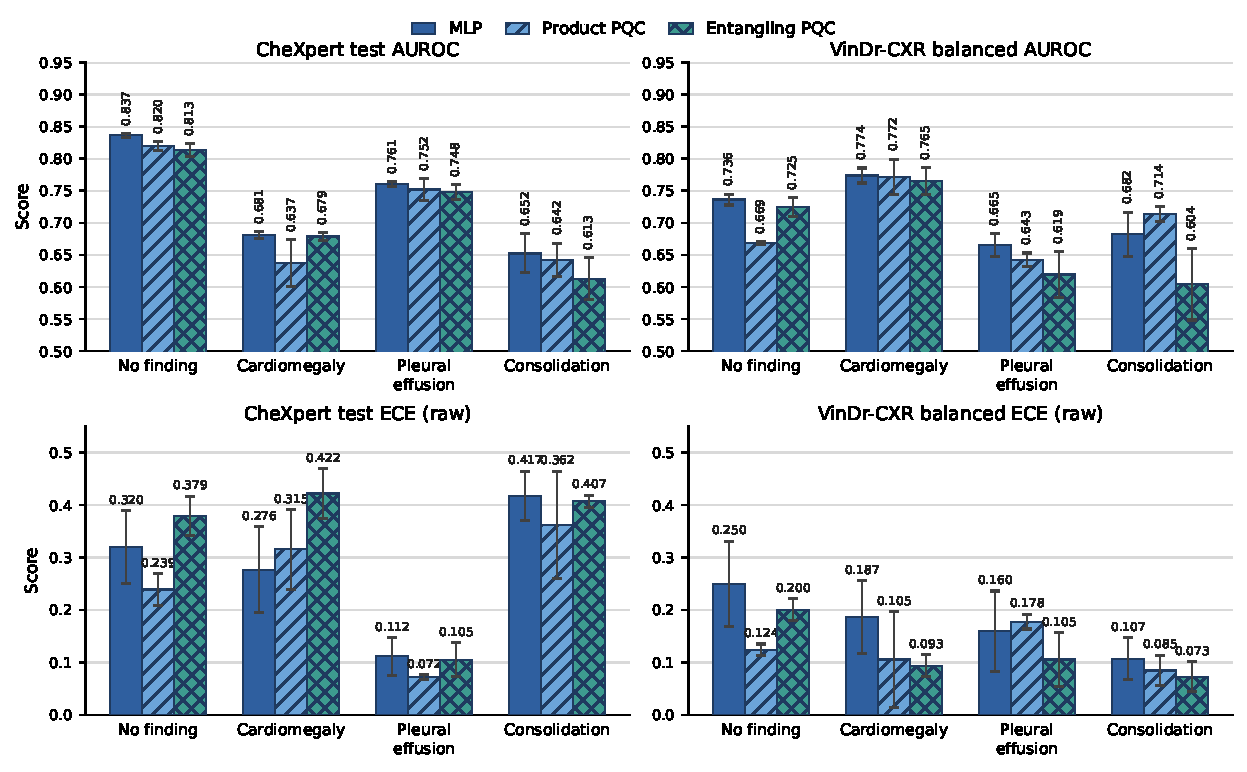
\includegraphics[width=\textwidth]{../results/figures/fig_auroc_ece_bars.pdf}
\caption{Matched-capacity heads on a frozen DenseNet-121 six-dimensional bottleneck. Bars are mean$\pm$std over three seeds. Discrimination is secondary; calibration is primary.}
\label{fig:bars}
\end{figure}

\begin{figure}[h]
\centering
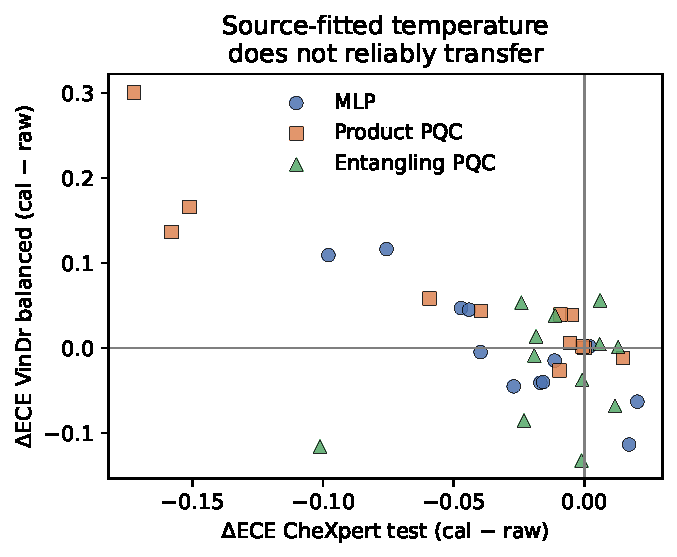
\includegraphics[width=0.62\textwidth]{../results/figures/fig_temperature_transfer.pdf}
\caption{Change in ECE after source-fitted temperature scaling. Points in the lower-left quadrant improve on both domains; points in the upper-left improve on CheXpert and degrade on VinDr-CXR.}
\label{fig:transfer}
\end{figure}

\begin{figure}[h]
\centering
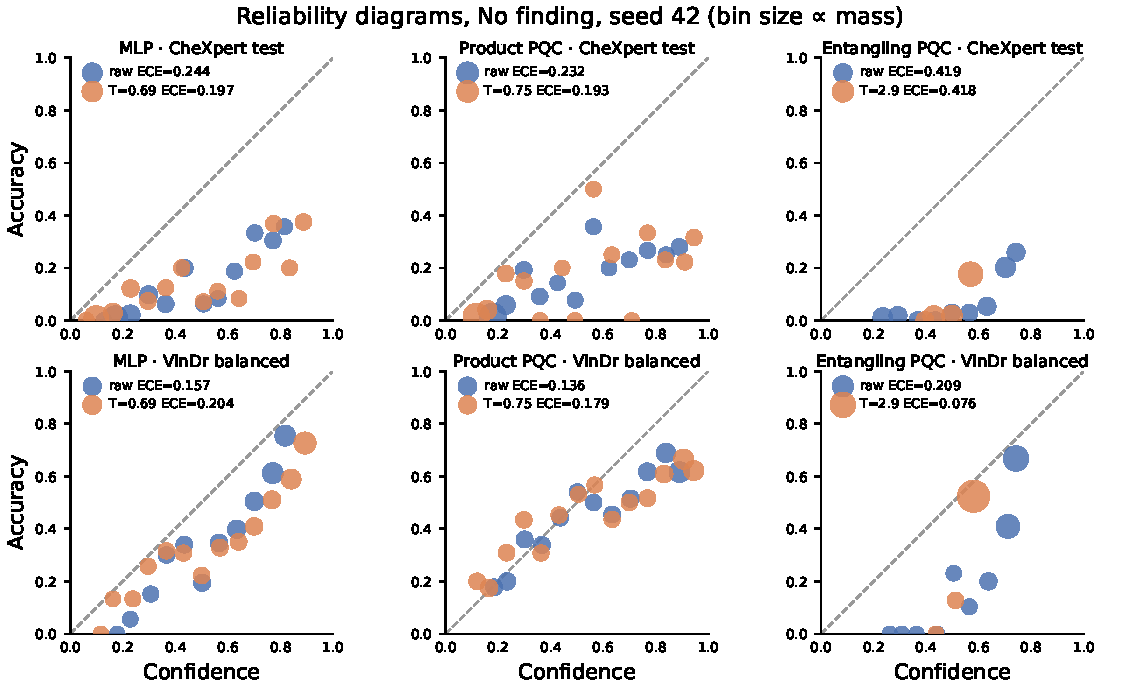
\includegraphics[width=\textwidth]{../results/figures/fig_reliability_no_finding_seed42.pdf}
\caption{Reliability diagrams for no finding, seed 42. Marker area is proportional to bin mass. Entangling PQC over-predicts the positive class on CheXpert test; temperature fitted on CheXpert validation does not restore a diagonal on VinDr-CXR for the product head.}
\label{fig:reliability}
\end{figure}

\end{document}
